\documentclass[../article.tex]{subfiles}

% Change defintion of input path
\makeatletter
\def\input@path{{../tex}}
\makeatother

\begin{document}
\validinsub{%
\title{\LaTeX Article Template}
\author{Siddharth Bhat}
\date{\today}

\maketitle
\clearpage
%
\tableofcontents%
\listoffigures%
\listoftables%
\clearpage%
}

\section{The First Section}

This is the main body of the ``First Section''. Here we have a referance
to `\verb|ref1|' \cite{ref1}.

\subsection{A subsection}

The is subsection text: \blindtext

\subsection{Yet Another Subsection}

This is the second subsection body. here we have another referance \cite{ref3}.

\section{Some Floats - Tables and Images}

\subsection{A table}

\begin{table}[H]
	\centering
	\begin{tabular}{ |l|l| }
	\hline
	\multicolumn{2}{|c|}{Team sheet} \\
	\hline
	GK & Paul Robinson \\
	LB & Lucas Radebe \\
	DC & Michael Duberry \\
	DC & Dominic Matteo \\
	RB & Dider Domi \\
	MC & David Batty \\
	MC & Eirik Bakke \\
	MC & Jody Morris \\
	FW & Jamie McMaster \\
	ST & Alan Smith \\
	ST & Mark Viduka \\
	\hline
	\end{tabular}
	\caption{A table}
\end{table}

\subsection{Some Images}

\begin{figure}[H]
	\centering
	\hfill
	\begin{subfigure}[b]{0.4\textwidth}
		\centering
		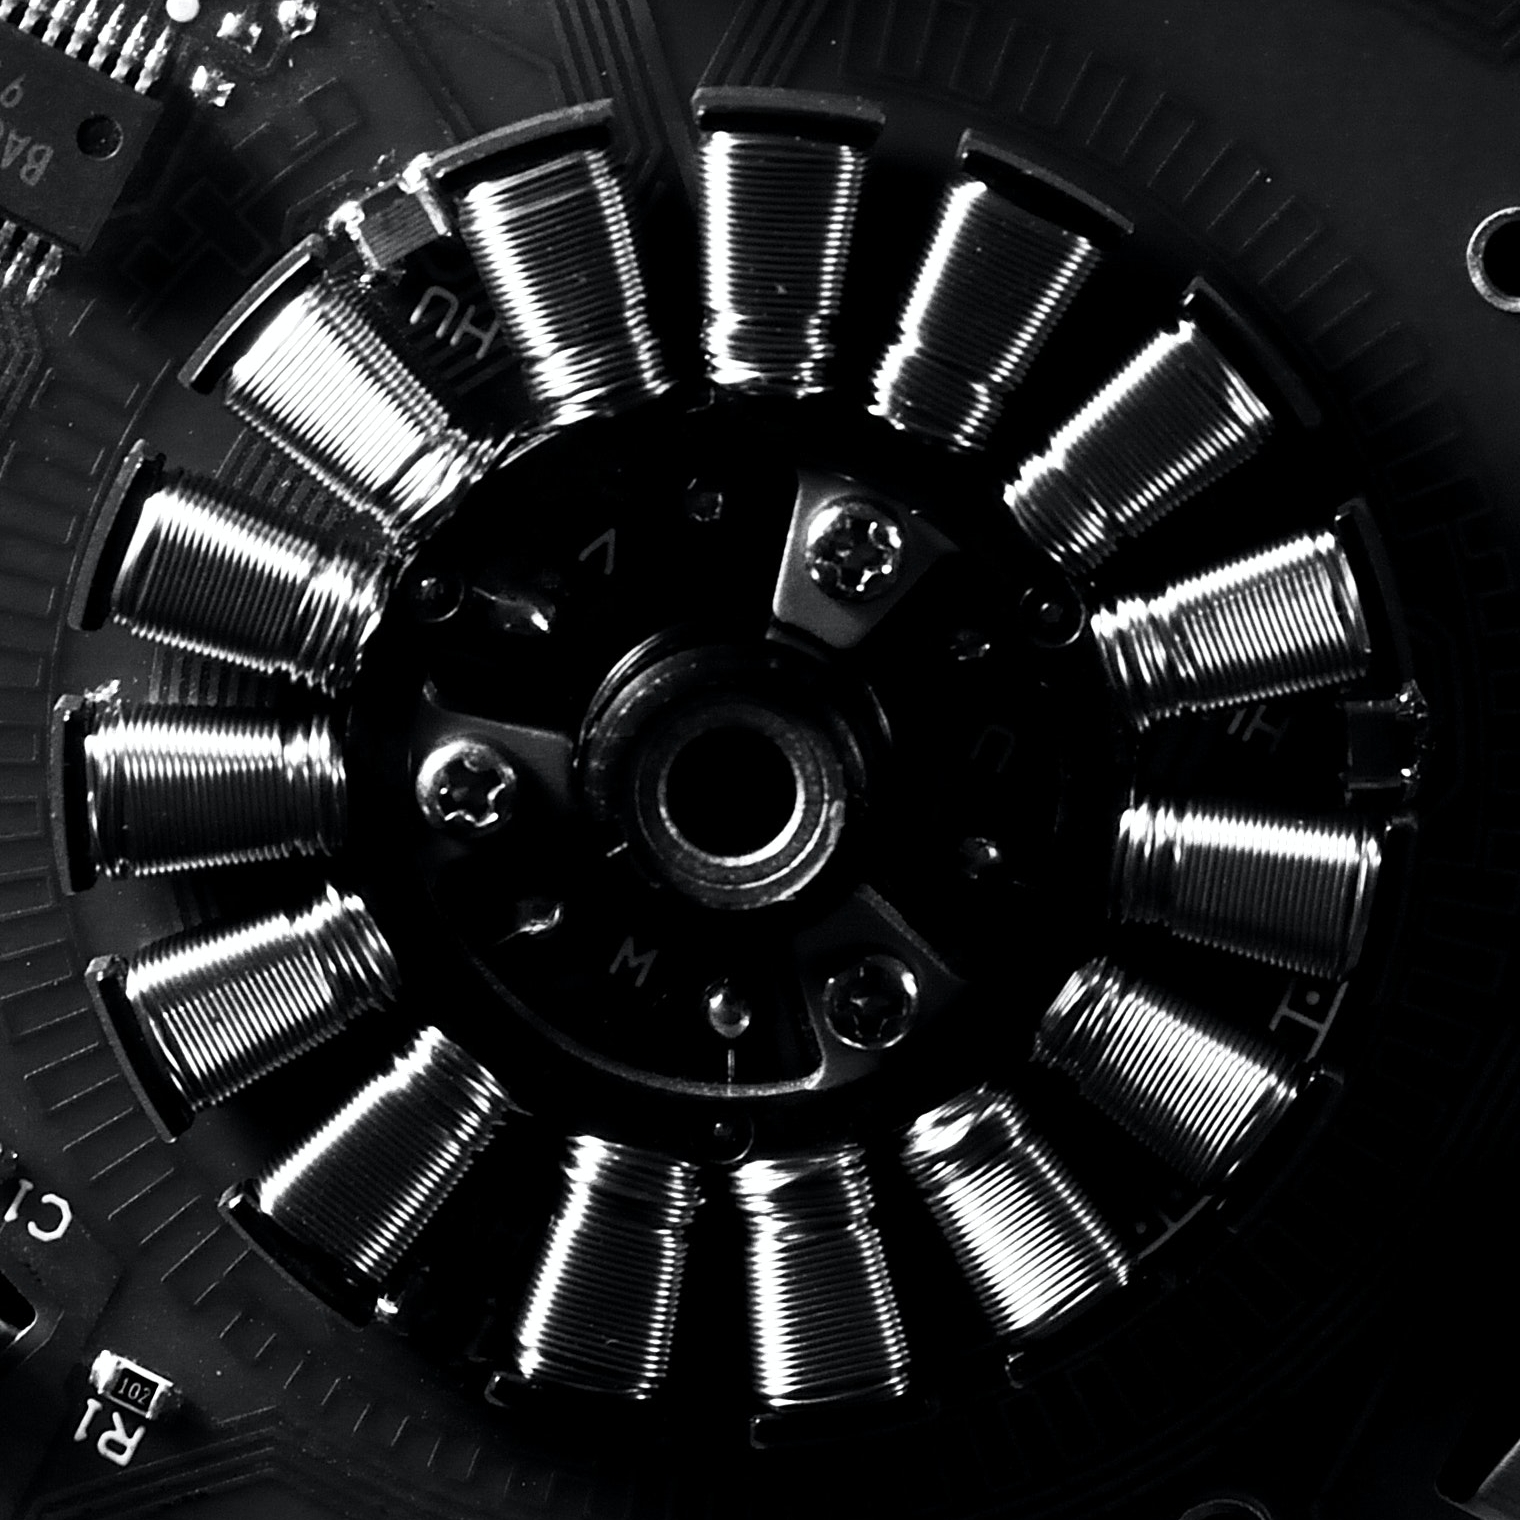
\includegraphics[width=\textwidth]{../images/image}
		\caption{\small Sub Image1}
	\end{subfigure}
	\hfill
	\begin{subfigure}[b]{0.4\textwidth}
		\centering
		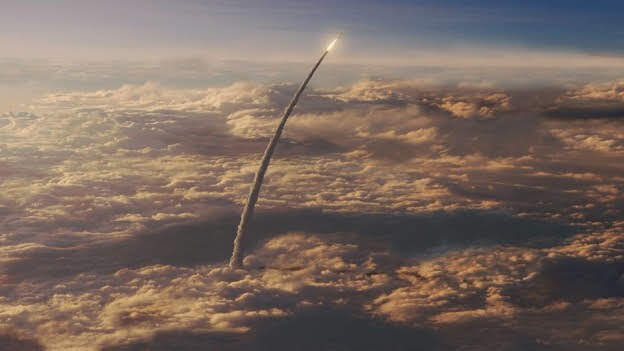
\includegraphics[width=\textwidth]{../images/image2}
		\caption{\small Sub Image2}
	\end{subfigure}
	\hfill
	\caption{Example of subfigures}
\end{figure}

\validinsub{% Bibliography Style
\bibliographystyle{plain}

% Costom Section Title
\renewcommand{\refname}{\section{Bibliography}} % Using "Bibliography" as the title of the section


% The Bibliography database
% You can define this in file or specify a 'bib' file
\validinmain{\bibliography{bibliography}}
\validinsub{\bibliography{../bibliography}}

%% In document style bibilography
% \begin{thebibliography}{9}
% 	\bibitem{ref1} Author Name, Work Title, Institute, Date
% 	\bibitem{ref2} Author2 Name2, Work Title2, Institute2, Date2
% 	\bibitem{ref3} Author3 Name3, Work Title3, Institute3, Date3
% 	\bibitem{ref4} Author4 Name4, Work Title4, Institute4, Date4
% \end{thebibliography}
}
\end{document}
